\lhead{\begin{minipage}{0.7\linewidth}
          \vspace{-12pt}\large Anlagen
    \end{minipage}}
    \addcontentsline{toc}{section}{Anlagen}
    \section*{Anlagen}\label{Anhang}
    
    \appendix
    \section{Aufnahmen für die Detektion auf dem Modell unbekannten Bildern}
    \label{app: Aufnahmen für die Detektion auf dem Modell unbekannten Bildern}
    
    \begin{figure}[htbp]
        \centering
        \includegraphics[width = 0.55\textwidth]{Bilder/misc/on_paper.jpg}
        \caption{Originalbild auf neutralem Hintergrund (Papier)}
        \label{fig:on_paper}
    \end{figure}
    
    \begin{figure}[htbp]
        \vspace{-1cm}
        \centering
        \includegraphics[width = 0.85\textwidth]{Bilder/misc/detection_on_paper.png}
        \caption{Bild nach Verkleinerung und Detektion auf neutralem Hintergrund (Papier)}
        \label{fig:det_on_paper}
    \end{figure}
    
    
    
    \begin{figure}[htbp]
        \centering
        \includegraphics[width = 0.6\textwidth]{Bilder/misc/on_wood.jpg}
        \caption{Originalbild auf Holztisch}
        \label{fig:on_wood}
    \end{figure}
    
    \begin{figure}[htbp]
        \vspace{-1cm}
        \centering
        \includegraphics[width = 0.9\textwidth]{Bilder/misc/detection_on_wood.png}
        \caption{Bild nach Verkleinerung und Detektion auf Holztisch}
        \label{fig:det_on_wood}
    \end{figure}
    
    
    
    
    
    
    
    \pagebreak
    
    \section{TensorBoard-Ausgaben für den Vergleich verschiedener Modelle}
    \label{app: TensorBoard-Ausgaben für den Vergleich verschiedener Modelle}
    
    \begin{figure}[H]
        \vspace{-0.027\textheight}
        \centering
        \includegraphics[angle = 90, height = 0.92\textheight]{Bilder/models/model_comparison/tensorboards/efficientdet_d1_coco17_tpu-32.png}
        \caption{TensorBoard-Ausgabe für das Modell \textit{efficientdet\_d1}}
        \label{fig:TensorBoard-1}
    \end{figure}
    
    \begin{figure}[H]
        \centering
        \includegraphics[angle = 90, height = 0.92\textheight]{Bilder/models/model_comparison/tensorboards/faster_rcnn_inception_resnet_v2_640x640_coco17_tpu-8.png}
        \caption{TensorBoard-Ausgabe für das Modell \textit{faster\_rcnn\_inception\_resnet\_v2}}
        \label{fig:TensorBoard-2}
    \end{figure}
    
    \begin{figure}[H]
        \centering
        \includegraphics[angle = 90, height = 0.92\textheight]{Bilder/models/model_comparison/tensorboards/faster_rcnn_resnet50_v1_640x640_coco17_tpu-8.png}
        \caption{TensorBoard-Ausgabe für das Modell \textit{faster\_rcnn\_resnet50\_v1}}
        \label{fig:TensorBoard-3}
    \end{figure}
    
    \begin{figure}[H]
        \centering
        \includegraphics[angle = 90, height = 0.92\textheight]{Bilder/models/model_comparison/tensorboards/faster_rcnn_resnet101_v1_640x640_coco17_tpu-8.png}
        \caption{TensorBoard-Ausgabe für das Modell \textit{faster\_rcnn\_resnet101\_v1}}
        \label{fig:TensorBoard-4}
    \end{figure}
    
    \begin{figure}[H]
        \centering
        \includegraphics[angle = 90, height = 0.92\textheight]{Bilder/models/model_comparison/tensorboards/ssd_mobilenet_v1_fpn_640x640_coco17_tpu-8.png}
        \caption{TensorBoard-Ausgabe für das Modell \textit{ssd\_mobilenet\_v1\_fpn}}
        \label{fig:TensorBoard-5}
    \end{figure}
    
    \begin{figure}[H]
        \centering
        \includegraphics[angle = 90, height = 0.92\textheight]{Bilder/models/model_comparison/tensorboards/ssd_mobilenet_v2_fpnlite_640x640_coco17_tpu-8.png}
        \caption{TensorBoard-Ausgabe für das Modell \textit{ssd\_mobilenet\_v2\_fpnlite}}
        \label{fig:TensorBoard-6}
    \end{figure}
    
    \begin{figure}[H]
        \centering
        \includegraphics[angle = 90, height = 0.92\textheight]{Bilder/models/model_comparison/tensorboards/ssd_resnet50_v1_fpn_640x640_coco17_tpu-8.png}
        \caption{TensorBoard-Ausgabe für das Modell \textit{ssd\_resnet50\_v1\_fpn}}
        \label{fig:TensorBoard-7}
    \end{figure}
    
    \begin{figure}[H]
        \centering
        \includegraphics[angle = 90, height = 0.92\textheight]{Bilder/models/model_comparison/tensorboards/ssd_resnet101_v1_fpn_640x640_coco17_tpu-8.png}
        \caption{TensorBoard-Ausgabe für das Modell \textit{ssd\_resnet101\_v1\_fpn}}
        \label{fig:TensorBoard-8}
    \end{figure}
    
    
    \section{Objekterkennung auf den Testbildern zum Vergleich der verschiedenen Modelle}
    \label{app: Objekterkennung auf den Testbildern zum Vergleich der verschiedenen Modelle}
    
    \subsection{Die Vorlagenbilder ohne Detektionen}
    
    \begin{figure}[H]
        \vspace{-5mm}
        \centering
        \includegraphics[angle = 90, height = 0.85\textheight]{Bilder/models/model_comparison/images-to-detect/trained_1.jpg}
        \caption{Mit trainiertes Bild 1 aus dem Datensatz mit niedriger Auflösung}
    \end{figure}
    
    \begin{figure}[H]
        \centering
        \includegraphics[angle = 90, width = \textwidth]{Bilder/models/model_comparison/images-to-detect/trained_2.jpg}
        \caption{Mit trainiertes Bild 2 aus dem Datensatz mit niedriger Auflösung}
    \end{figure}
    
    \begin{figure}[H]
        \centering
        \includegraphics[angle = 90, width = \textwidth]{Bilder/models/model_comparison/images-to-detect/trained_3.jpg}
        \caption{Mit trainiertes Bild 3 aus dem Datensatz mit niedriger Auflösung}
    \end{figure}
    
    \begin{figure}[H]
        \centering
        \includegraphics[angle = 90, width = \textwidth]{Bilder/models/model_comparison/images-to-detect/non_trained_1.jpg}
        \caption{Nicht trainiertes Bild 1 aus dem Datensatz mit niedriger Auflösung}
    \end{figure}
    
    \begin{figure}[H]
        \centering
        \includegraphics[angle = 90, width = \textwidth]{Bilder/models/model_comparison/images-to-detect/non_trained_2.jpg}
        \caption{Nicht trainiertes Bild 2 aus dem Datensatz mit niedriger Auflösung}
    \end{figure}
    
    \begin{figure}[H]
        \centering
        \includegraphics[angle = 90, width = \textwidth]{Bilder/models/model_comparison/images-to-detect/non_trained_3.jpg}
        \caption{Nicht trainiertes Bild 3 aus dem Datensatz mit niedriger Auflösung}
    \end{figure}
    
    \begin{figure}[H]
        \centering
        \includegraphics[angle = 90, width = \textwidth]{Bilder/models/model_comparison/images-to-detect/HD_on_white.jpg}
        \caption{Nicht trainiertes Bild mit hoher Auflösung auf weißem Hintergrund}
    \end{figure}
    
    \begin{figure}[H]
        \centering
        \includegraphics[angle = 90, width = \textwidth]{Bilder/models/model_comparison/images-to-detect/HD_on_doormat.jpg}
        \caption{Nicht trainiertes Bild mit hoher Auflösung auf Fußmatte als Hintergrund}
    \end{figure}
    
    \begin{figure}[H]
        \centering
        \includegraphics[angle = 90, width = \textwidth]{Bilder/models/model_comparison/images-to-detect/HD_on_granite.jpg}
        \caption{Nicht trainiertes Bild mit hoher Auflösung auf Granit als Hintergrund}
    \end{figure}
    
    \begin{figure}[H]
        \centering
        \includegraphics[angle = 90, width = \textwidth]{Bilder/models/model_comparison/images-to-detect/HD_on_marble.jpg}
        \caption{Nicht trainiertes Bild mit hoher Auflösung auf marmoriertem Hintergrund}
    \end{figure}
    
    \begin{figure}[H]
        \centering
        \includegraphics[angle = 90, width = \textwidth]{Bilder/models/model_comparison/images-to-detect/HD_on_wood.jpg}
        \caption{Nicht trainiertes Bild mit hoher Auflösung auf Holztisch als Hintergrund}
    \end{figure}
    
    
    \subsection{Die Detektionen durch das \textit{efficientdet}-Modell}
    
    \begin{figure}[H]
        \vspace{-5mm}
        \centering
        \includegraphics[angle = 90, height = 0.85\textheight]{Bilder/models/model_comparison/efficientdet_d1_coco17_tpu-32/trained_1.jpg}
        \caption{Mit trainiertes Bild 1 aus dem Datensatz mit niedriger Auflösung}
    \end{figure}
    
    \begin{figure}[H]
        \centering
        \includegraphics[angle = 90, width = \textwidth]{Bilder/models/model_comparison/efficientdet_d1_coco17_tpu-32/trained_2.jpg}
        \caption{Mit trainiertes Bild 2 aus dem Datensatz mit niedriger Auflösung}
    \end{figure}
    
    \begin{figure}[H]
        \centering
        \includegraphics[angle = 90, width = \textwidth]{Bilder/models/model_comparison/efficientdet_d1_coco17_tpu-32/trained_3.jpg}
        \caption{Mit trainiertes Bild 3 aus dem Datensatz mit niedriger Auflösung}
    \end{figure}
    
    \begin{figure}[H]
        \centering
        \includegraphics[angle = 90, width = \textwidth]{Bilder/models/model_comparison/efficientdet_d1_coco17_tpu-32/non_trained_1.jpg}
        \caption{Nicht trainiertes Bild 1 aus dem Datensatz mit niedriger Auflösung}
    \end{figure}
    
    \begin{figure}[H]
        \centering
        \includegraphics[angle = 90, width = \textwidth]{Bilder/models/model_comparison/efficientdet_d1_coco17_tpu-32/non_trained_2.jpg}
        \caption{Nicht trainiertes Bild 2 aus dem Datensatz mit niedriger Auflösung}
    \end{figure}
    
    \begin{figure}[H]
        \centering
        \includegraphics[angle = 90, width = \textwidth]{Bilder/models/model_comparison/efficientdet_d1_coco17_tpu-32/non_trained_3.jpg}
        \caption{Nicht trainiertes Bild 3 aus dem Datensatz mit niedriger Auflösung}
    \end{figure}
    
    \begin{figure}[H]
        \centering
        \includegraphics[angle = 90, width = \textwidth]{Bilder/models/model_comparison/efficientdet_d1_coco17_tpu-32/HD_on_white.jpg}
        \caption{Nicht trainiertes Bild mit hoher Auflösung auf weißem Hintergrund}
    \end{figure}
    
    \begin{figure}[H]
        \centering
        \includegraphics[angle = 90, width = \textwidth]{Bilder/models/model_comparison/efficientdet_d1_coco17_tpu-32/HD_on_doormat.jpg}
        \caption{Nicht trainiertes Bild mit hoher Auflösung auf Fußmatte als Hintergrund}
    \end{figure}
    
    \begin{figure}[H]
        \centering
        \includegraphics[angle = 90, width = \textwidth]{Bilder/models/model_comparison/efficientdet_d1_coco17_tpu-32/HD_on_granite.jpg}
        \caption{Nicht trainiertes Bild mit hoher Auflösung auf Granit als Hintergrund}
    \end{figure}
    
    \begin{figure}[H]
        \centering
        \includegraphics[angle = 90, width = \textwidth]{Bilder/models/model_comparison/efficientdet_d1_coco17_tpu-32/HD_on_marble.jpg}
        \caption{Nicht trainiertes Bild mit hoher Auflösung auf marmoriertem Hintergrund}
    \end{figure}
    
    \begin{figure}[H]
        \centering
        \includegraphics[angle = 90, width = \textwidth]{Bilder/models/model_comparison/efficientdet_d1_coco17_tpu-32/HD_on_wood.jpg}
        \caption{Nicht trainiertes Bild mit hoher Auflösung auf Holztisch als Hintergrund}
    \end{figure}
    
    \subsection{Die Detektionen durch das \textit{faster\_rcnn\_inception}-Modell}
    
    \begin{figure}[H]
        \vspace{-5mm}
        \centering
        \includegraphics[angle = 90, height = 0.85\textheight]{Bilder/models/model_comparison/faster_rcnn_inception_resnet_v2_640x640_coco17_tpu-8/trained_1.jpg}
        \caption{Mit trainiertes Bild 1 aus dem Datensatz mit niedriger Auflösung}
    \end{figure}
    
    \begin{figure}[H]
        \centering
        \includegraphics[angle = 90, width = \textwidth]{Bilder/models/model_comparison/faster_rcnn_inception_resnet_v2_640x640_coco17_tpu-8/trained_2.jpg}
        \caption{Mit trainiertes Bild 2 aus dem Datensatz mit niedriger Auflösung}
    \end{figure}
    
    \begin{figure}[H]
        \centering
        \includegraphics[angle = 90, width = \textwidth]{Bilder/models/model_comparison/faster_rcnn_inception_resnet_v2_640x640_coco17_tpu-8/trained_3.jpg}
        \caption{Mit trainiertes Bild 3 aus dem Datensatz mit niedriger Auflösung}
    \end{figure}
    
    \begin{figure}[H]
        \centering
        \includegraphics[angle = 90, width = \textwidth]{Bilder/models/model_comparison/faster_rcnn_inception_resnet_v2_640x640_coco17_tpu-8/non_trained_1.jpg}
        \caption{Nicht trainiertes Bild 1 aus dem Datensatz mit niedriger Auflösung}
    \end{figure}
    
    \begin{figure}[H]
        \centering
        \includegraphics[angle = 90, width = \textwidth]{Bilder/models/model_comparison/faster_rcnn_inception_resnet_v2_640x640_coco17_tpu-8/non_trained_2.jpg}
        \caption{Nicht trainiertes Bild 2 aus dem Datensatz mit niedriger Auflösung}
    \end{figure}
    
    \begin{figure}[H]
        \centering
        \includegraphics[angle = 90, width = \textwidth]{Bilder/models/model_comparison/faster_rcnn_inception_resnet_v2_640x640_coco17_tpu-8/non_trained_3.jpg}
        \caption{Nicht trainiertes Bild 3 aus dem Datensatz mit niedriger Auflösung}
    \end{figure}
    
    \begin{figure}[H]
        \centering
        \includegraphics[angle = 90, width = \textwidth]{Bilder/models/model_comparison/faster_rcnn_inception_resnet_v2_640x640_coco17_tpu-8/HD_on_white.jpg}
        \caption{Nicht trainiertes Bild mit hoher Auflösung auf weißem Hintergrund}
    \end{figure}
    
    \begin{figure}[H]
        \centering
        \includegraphics[angle = 90, width = \textwidth]{Bilder/models/model_comparison/faster_rcnn_inception_resnet_v2_640x640_coco17_tpu-8/HD_on_doormat.jpg}
        \caption{Nicht trainiertes Bild mit hoher Auflösung auf Fußmatte als Hintergrund}
    \end{figure}
    
    \begin{figure}[H]
        \centering
        \includegraphics[angle = 90, width = \textwidth]{Bilder/models/model_comparison/faster_rcnn_inception_resnet_v2_640x640_coco17_tpu-8/HD_on_granite.jpg}
        \caption{Nicht trainiertes Bild mit hoher Auflösung auf Granit als Hintergrund}
    \end{figure}
    
    \begin{figure}[H]
        \centering
        \includegraphics[angle = 90, width = \textwidth]{Bilder/models/model_comparison/faster_rcnn_inception_resnet_v2_640x640_coco17_tpu-8/HD_on_marble.jpg}
        \caption{Nicht trainiertes Bild mit hoher Auflösung auf marmoriertem Hintergrund}
    \end{figure}
    
    \begin{figure}[H]
        \centering
        \includegraphics[angle = 90, width = \textwidth]{Bilder/models/model_comparison/faster_rcnn_inception_resnet_v2_640x640_coco17_tpu-8/HD_on_wood.jpg}
        \caption{Nicht trainiertes Bild mit hoher Auflösung auf Holztisch als Hintergrund}
    \end{figure}
    
    \subsection{Die Detektionen durch das \textit{faster\_rcnn\_resnet50}-Modell}
    
    \begin{figure}[H]
        \vspace{-5mm}
        \centering
        \includegraphics[angle = 90, height = 0.85\textheight]{Bilder/models/model_comparison/faster_rcnn_resnet50_v1_640x640_coco17_tpu-8/trained_1.jpg}
        \caption{Mit trainiertes Bild 1 aus dem Datensatz mit niedriger Auflösung}
    \end{figure}
    
    \begin{figure}[H]
        \centering
        \includegraphics[angle = 90, width = \textwidth]{Bilder/models/model_comparison/faster_rcnn_resnet50_v1_640x640_coco17_tpu-8/trained_2.jpg}
        \caption{Mit trainiertes Bild 2 aus dem Datensatz mit niedriger Auflösung}
    \end{figure}
    
    \begin{figure}[H]
        \centering
        \includegraphics[angle = 90, width = \textwidth]{Bilder/models/model_comparison/faster_rcnn_resnet50_v1_640x640_coco17_tpu-8/trained_3.jpg}
        \caption{Mit trainiertes Bild 3 aus dem Datensatz mit niedriger Auflösung}
    \end{figure}
    
    \begin{figure}[H]
        \centering
        \includegraphics[angle = 90, width = \textwidth]{Bilder/models/model_comparison/faster_rcnn_resnet50_v1_640x640_coco17_tpu-8/non_trained_1.jpg}
        \caption{Nicht trainiertes Bild 1 aus dem Datensatz mit niedriger Auflösung}
    \end{figure}
    
    \begin{figure}[H]
        \centering
        \includegraphics[angle = 90, width = \textwidth]{Bilder/models/model_comparison/faster_rcnn_resnet50_v1_640x640_coco17_tpu-8/non_trained_2.jpg}
        \caption{Nicht trainiertes Bild 2 aus dem Datensatz mit niedriger Auflösung}
    \end{figure}
    
    \begin{figure}[H]
        \centering
        \includegraphics[angle = 90, width = \textwidth]{Bilder/models/model_comparison/faster_rcnn_resnet50_v1_640x640_coco17_tpu-8/non_trained_3.jpg}
        \caption{Nicht trainiertes Bild 3 aus dem Datensatz mit niedriger Auflösung}
    \end{figure}
    
    \begin{figure}[H]
        \centering
        \includegraphics[angle = 90, width = \textwidth]{Bilder/models/model_comparison/faster_rcnn_resnet50_v1_640x640_coco17_tpu-8/HD_on_white.jpg}
        \caption{Nicht trainiertes Bild mit hoher Auflösung auf weißem Hintergrund}
    \end{figure}
    
    \begin{figure}[H]
        \centering
        \includegraphics[angle = 90, width = \textwidth]{Bilder/models/model_comparison/faster_rcnn_resnet50_v1_640x640_coco17_tpu-8/HD_on_doormat.jpg}
        \caption{Nicht trainiertes Bild mit hoher Auflösung auf Fußmatte als Hintergrund}
    \end{figure}
    
    \begin{figure}[H]
        \centering
        \includegraphics[angle = 90, width = \textwidth]{Bilder/models/model_comparison/faster_rcnn_resnet50_v1_640x640_coco17_tpu-8/HD_on_granite.jpg}
        \caption{Nicht trainiertes Bild mit hoher Auflösung auf Granit als Hintergrund}
    \end{figure}
    
    \begin{figure}[H]
        \centering
        \includegraphics[angle = 90, width = \textwidth]{Bilder/models/model_comparison/faster_rcnn_resnet50_v1_640x640_coco17_tpu-8/HD_on_marble.jpg}
        \caption{Nicht trainiertes Bild mit hoher Auflösung auf marmoriertem Hintergrund}
    \end{figure}
    
    \begin{figure}[H]
        \centering
        \includegraphics[angle = 90, width = \textwidth]{Bilder/models/model_comparison/faster_rcnn_resnet50_v1_640x640_coco17_tpu-8/HD_on_wood.jpg}
        \caption{Nicht trainiertes Bild mit hoher Auflösung auf Holztisch als Hintergrund}
    \end{figure}
    
    \subsection{Die Detektionen durch das \textit{faster\_rcnn\_resnet101}-Modell}
    
    \begin{figure}[H]
        \vspace{-5mm}
        \centering
        \includegraphics[angle = 90, height = 0.85\textheight]{Bilder/models/model_comparison/faster_rcnn_resnet101_v1_640x640_coco17_tpu-8/trained_1.jpg}
        \caption{Mit trainiertes Bild 1 aus dem Datensatz mit niedriger Auflösung}
    \end{figure}
    
    \begin{figure}[H]
        \centering
        \includegraphics[angle = 90, width = \textwidth]{Bilder/models/model_comparison/faster_rcnn_resnet101_v1_640x640_coco17_tpu-8/trained_2.jpg}
        \caption{Mit trainiertes Bild 2 aus dem Datensatz mit niedriger Auflösung}
    \end{figure}
    
    \begin{figure}[H]
        \centering
        \includegraphics[angle = 90, width = \textwidth]{Bilder/models/model_comparison/faster_rcnn_resnet101_v1_640x640_coco17_tpu-8/trained_3.jpg}
        \caption{Mit trainiertes Bild 3 aus dem Datensatz mit niedriger Auflösung}
    \end{figure}
    
    \begin{figure}[H]
        \centering
        \includegraphics[angle = 90, width = \textwidth]{Bilder/models/model_comparison/faster_rcnn_resnet101_v1_640x640_coco17_tpu-8/non_trained_1.jpg}
        \caption{Nicht trainiertes Bild 1 aus dem Datensatz mit niedriger Auflösung}
    \end{figure}
    
    \begin{figure}[H]
        \centering
        \includegraphics[angle = 90, width = \textwidth]{Bilder/models/model_comparison/faster_rcnn_resnet101_v1_640x640_coco17_tpu-8/non_trained_2.jpg}
        \caption{Nicht trainiertes Bild 2 aus dem Datensatz mit niedriger Auflösung}
    \end{figure}
    
    \begin{figure}[H]
        \centering
        \includegraphics[angle = 90, width = \textwidth]{Bilder/models/model_comparison/faster_rcnn_resnet101_v1_640x640_coco17_tpu-8/non_trained_3.jpg}
        \caption{Nicht trainiertes Bild 3 aus dem Datensatz mit niedriger Auflösung}
    \end{figure}
    
    \begin{figure}[H]
        \centering
        \includegraphics[angle = 90, width = \textwidth]{Bilder/models/model_comparison/faster_rcnn_resnet101_v1_640x640_coco17_tpu-8/HD_on_white.jpg}
        \caption{Nicht trainiertes Bild mit hoher Auflösung auf weißem Hintergrund}
    \end{figure}
    
    \begin{figure}[H]
        \centering
        \includegraphics[angle = 90, width = \textwidth]{Bilder/models/model_comparison/faster_rcnn_resnet101_v1_640x640_coco17_tpu-8/HD_on_doormat.jpg}
        \caption{Nicht trainiertes Bild mit hoher Auflösung auf Fußmatte als Hintergrund}
    \end{figure}
    
    \begin{figure}[H]
        \centering
        \includegraphics[angle = 90, width = \textwidth]{Bilder/models/model_comparison/faster_rcnn_resnet101_v1_640x640_coco17_tpu-8/HD_on_granite.jpg}
        \caption{Nicht trainiertes Bild mit hoher Auflösung auf Granit als Hintergrund}
    \end{figure}
    
    \begin{figure}[H]
        \centering
        \includegraphics[angle = 90, width = \textwidth]{Bilder/models/model_comparison/faster_rcnn_resnet101_v1_640x640_coco17_tpu-8/HD_on_marble.jpg}
        \caption{Nicht trainiertes Bild mit hoher Auflösung auf marmoriertem Hintergrund}
    \end{figure}
    
    \begin{figure}[H]
        \centering
        \includegraphics[angle = 90, width = \textwidth]{Bilder/models/model_comparison/faster_rcnn_resnet101_v1_640x640_coco17_tpu-8/HD_on_wood.jpg}
        \caption{Nicht trainiertes Bild mit hoher Auflösung auf Holztisch als Hintergrund}
    \end{figure}
    
    \subsection{Die Detektionen durch das \textit{ssd\_mobilenet\_v1}-Modell}
    
    \begin{figure}[H]
        \vspace{-5mm}
        \centering
        \includegraphics[angle = 90, height = 0.85\textheight]{Bilder/models/model_comparison/ssd_mobilenet_v1_fpn_640x640_coco17_tpu-8/trained_1.jpg}
        \caption{Mit trainiertes Bild 1 aus dem Datensatz mit niedriger Auflösung}
    \end{figure}
    
    \begin{figure}[H]
        \centering
        \includegraphics[angle = 90, width = \textwidth]{Bilder/models/model_comparison/ssd_mobilenet_v1_fpn_640x640_coco17_tpu-8/trained_2.jpg}
        \caption{Mit trainiertes Bild 2 aus dem Datensatz mit niedriger Auflösung}
    \end{figure}
    
    \begin{figure}[H]
        \centering
        \includegraphics[angle = 90, width = \textwidth]{Bilder/models/model_comparison/ssd_mobilenet_v1_fpn_640x640_coco17_tpu-8/trained_3.jpg}
        \caption{Mit trainiertes Bild 3 aus dem Datensatz mit niedriger Auflösung}
    \end{figure}
    
    \begin{figure}[H]
        \centering
        \includegraphics[angle = 90, width = \textwidth]{Bilder/models/model_comparison/ssd_mobilenet_v1_fpn_640x640_coco17_tpu-8/non_trained_1.jpg}
        \caption{Nicht trainiertes Bild 1 aus dem Datensatz mit niedriger Auflösung}
    \end{figure}
    
    \begin{figure}[H]
        \centering
        \includegraphics[angle = 90, width = \textwidth]{Bilder/models/model_comparison/ssd_mobilenet_v1_fpn_640x640_coco17_tpu-8/non_trained_2.jpg}
        \caption{Nicht trainiertes Bild 2 aus dem Datensatz mit niedriger Auflösung}
    \end{figure}
    
    \begin{figure}[H]
        \centering
        \includegraphics[angle = 90, width = \textwidth]{Bilder/models/model_comparison/ssd_mobilenet_v1_fpn_640x640_coco17_tpu-8/non_trained_3.jpg}
        \caption{Nicht trainiertes Bild 3 aus dem Datensatz mit niedriger Auflösung}
    \end{figure}
    
    \begin{figure}[H]
        \centering
        \includegraphics[angle = 90, width = \textwidth]{Bilder/models/model_comparison/ssd_mobilenet_v1_fpn_640x640_coco17_tpu-8/HD_on_white.jpg}
        \caption{Nicht trainiertes Bild mit hoher Auflösung auf weißem Hintergrund}
    \end{figure}
    
    \begin{figure}[H]
        \centering
        \includegraphics[angle = 90, width = \textwidth]{Bilder/models/model_comparison/ssd_mobilenet_v1_fpn_640x640_coco17_tpu-8/HD_on_doormat.jpg}
        \caption{Nicht trainiertes Bild mit hoher Auflösung auf Fußmatte als Hintergrund}
    \end{figure}
    
    \begin{figure}[H]
        \centering
        \includegraphics[angle = 90, width = \textwidth]{Bilder/models/model_comparison/ssd_mobilenet_v1_fpn_640x640_coco17_tpu-8/HD_on_granite.jpg}
        \caption{Nicht trainiertes Bild mit hoher Auflösung auf Granit als Hintergrund}
    \end{figure}
    
    \begin{figure}[H]
        \centering
        \includegraphics[angle = 90, width = \textwidth]{Bilder/models/model_comparison/ssd_mobilenet_v1_fpn_640x640_coco17_tpu-8/HD_on_marble.jpg}
        \caption{Nicht trainiertes Bild mit hoher Auflösung auf marmoriertem Hintergrund}
    \end{figure}
    
    \begin{figure}[H]
        \centering
        \includegraphics[angle = 90, width = \textwidth]{Bilder/models/model_comparison/ssd_mobilenet_v1_fpn_640x640_coco17_tpu-8/HD_on_wood.jpg}
        \caption{Nicht trainiertes Bild mit hoher Auflösung auf Holztisch als Hintergrund}
    \end{figure}
    
    \subsection{Die Detektionen durch das \textit{ssd\_mobilenet\_v2}-Modell}
    
    \begin{figure}[H]
        \vspace{-5mm}
        \centering
        \includegraphics[angle = 90, height = 0.85\textheight]{Bilder/models/model_comparison/ssd_mobilenet_v2_fpnlite_640x640_coco17_tpu-8/trained_1.jpg}
        \caption{Mit trainiertes Bild 1 aus dem Datensatz mit niedriger Auflösung}
    \end{figure}
    
    \begin{figure}[H]
        \centering
        \includegraphics[angle = 90, width = \textwidth]{Bilder/models/model_comparison/ssd_mobilenet_v2_fpnlite_640x640_coco17_tpu-8/trained_2.jpg}
        \caption{Mit trainiertes Bild 2 aus dem Datensatz mit niedriger Auflösung}
    \end{figure}
    
    \begin{figure}[H]
        \centering
        \includegraphics[angle = 90, width = \textwidth]{Bilder/models/model_comparison/ssd_mobilenet_v2_fpnlite_640x640_coco17_tpu-8/trained_3.jpg}
        \caption{Mit trainiertes Bild 3 aus dem Datensatz mit niedriger Auflösung}
    \end{figure}
    
    \begin{figure}[H]
        \centering
        \includegraphics[angle = 90, width = \textwidth]{Bilder/models/model_comparison/ssd_mobilenet_v2_fpnlite_640x640_coco17_tpu-8/non_trained_1.jpg}
        \caption{Nicht trainiertes Bild 1 aus dem Datensatz mit niedriger Auflösung}
    \end{figure}
    
    \begin{figure}[H]
        \centering
        \includegraphics[angle = 90, width = \textwidth]{Bilder/models/model_comparison/ssd_mobilenet_v2_fpnlite_640x640_coco17_tpu-8/non_trained_2.jpg}
        \caption{Nicht trainiertes Bild 2 aus dem Datensatz mit niedriger Auflösung}
    \end{figure}
    
    \begin{figure}[H]
        \centering
        \includegraphics[angle = 90, width = \textwidth]{Bilder/models/model_comparison/ssd_mobilenet_v2_fpnlite_640x640_coco17_tpu-8/non_trained_3.jpg}
        \caption{Nicht trainiertes Bild 3 aus dem Datensatz mit niedriger Auflösung}
    \end{figure}
    
    \begin{figure}[H]
        \centering
        \includegraphics[angle = 90, width = \textwidth]{Bilder/models/model_comparison/ssd_mobilenet_v2_fpnlite_640x640_coco17_tpu-8/HD_on_white.jpg}
        \caption{Nicht trainiertes Bild mit hoher Auflösung auf weißem Hintergrund}
    \end{figure}
    
    \begin{figure}[H]
        \centering
        \includegraphics[angle = 90, width = \textwidth]{Bilder/models/model_comparison/ssd_mobilenet_v2_fpnlite_640x640_coco17_tpu-8/HD_on_doormat.jpg}
        \caption{Nicht trainiertes Bild mit hoher Auflösung auf Fußmatte als Hintergrund}
    \end{figure}
    
    \begin{figure}[H]
        \centering
        \includegraphics[angle = 90, width = \textwidth]{Bilder/models/model_comparison/ssd_mobilenet_v2_fpnlite_640x640_coco17_tpu-8/HD_on_granite.jpg}
        \caption{Nicht trainiertes Bild mit hoher Auflösung auf Granit als Hintergrund}
    \end{figure}
    
    \begin{figure}[H]
        \centering
        \includegraphics[angle = 90, width = \textwidth]{Bilder/models/model_comparison/ssd_mobilenet_v2_fpnlite_640x640_coco17_tpu-8/HD_on_marble.jpg}
        \caption{Nicht trainiertes Bild mit hoher Auflösung auf marmoriertem Hintergrund}
    \end{figure}
    
    \begin{figure}[H]
        \centering
        \includegraphics[angle = 90, width = \textwidth]{Bilder/models/model_comparison/ssd_mobilenet_v2_fpnlite_640x640_coco17_tpu-8/HD_on_wood.jpg}
        \caption{Nicht trainiertes Bild mit hoher Auflösung auf Holztisch als Hintergrund}
    \end{figure}
    
    \subsection{Die Detektionen durch das \textit{ssd\_resnet50}-Modell}
    
    \begin{figure}[H]
        \vspace{-5mm}
        \centering
        \includegraphics[angle = 90, height = 0.85\textheight]{Bilder/models/model_comparison/ssd_resnet50_v1_fpn_640x640_coco17_tpu-8/trained_1.jpg}
        \caption{Mit trainiertes Bild 1 aus dem Datensatz mit niedriger Auflösung}
    \end{figure}
    
    \begin{figure}[H]
        \centering
        \includegraphics[angle = 90, width = \textwidth]{Bilder/models/model_comparison/ssd_resnet50_v1_fpn_640x640_coco17_tpu-8/trained_2.jpg}
        \caption{Mit trainiertes Bild 2 aus dem Datensatz mit niedriger Auflösung}
    \end{figure}
    
    \begin{figure}[H]
        \centering
        \includegraphics[angle = 90, width = \textwidth]{Bilder/models/model_comparison/ssd_resnet50_v1_fpn_640x640_coco17_tpu-8/trained_3.jpg}
        \caption{Mit trainiertes Bild 3 aus dem Datensatz mit niedriger Auflösung}
    \end{figure}
    
    \begin{figure}[H]
        \centering
        \includegraphics[angle = 90, width = \textwidth]{Bilder/models/model_comparison/ssd_resnet50_v1_fpn_640x640_coco17_tpu-8/non_trained_1.jpg}
        \caption{Nicht trainiertes Bild 1 aus dem Datensatz mit niedriger Auflösung}
    \end{figure}
    
    \begin{figure}[H]
        \centering
        \includegraphics[angle = 90, width = \textwidth]{Bilder/models/model_comparison/ssd_resnet50_v1_fpn_640x640_coco17_tpu-8/non_trained_2.jpg}
        \caption{Nicht trainiertes Bild 2 aus dem Datensatz mit niedriger Auflösung}
    \end{figure}
    
    \begin{figure}[H]
        \centering
        \includegraphics[angle = 90, width = \textwidth]{Bilder/models/model_comparison/ssd_resnet50_v1_fpn_640x640_coco17_tpu-8/non_trained_3.jpg}
        \caption{Nicht trainiertes Bild 3 aus dem Datensatz mit niedriger Auflösung}
    \end{figure}
    
    \begin{figure}[H]
        \centering
        \includegraphics[angle = 90, width = \textwidth]{Bilder/models/model_comparison/ssd_resnet50_v1_fpn_640x640_coco17_tpu-8/HD_on_white.jpg}
        \caption{Nicht trainiertes Bild mit hoher Auflösung auf weißem Hintergrund}
    \end{figure}
    
    \begin{figure}[H]
        \centering
        \includegraphics[angle = 90, width = \textwidth]{Bilder/models/model_comparison/ssd_resnet50_v1_fpn_640x640_coco17_tpu-8/HD_on_doormat.jpg}
        \caption{Nicht trainiertes Bild mit hoher Auflösung auf Fußmatte als Hintergrund}
    \end{figure}
    
    \begin{figure}[H]
        \centering
        \includegraphics[angle = 90, width = \textwidth]{Bilder/models/model_comparison/ssd_resnet50_v1_fpn_640x640_coco17_tpu-8/HD_on_granite.jpg}
        \caption{Nicht trainiertes Bild mit hoher Auflösung auf Granit als Hintergrund}
    \end{figure}
    
    \begin{figure}[H]
        \centering
        \includegraphics[angle = 90, width = \textwidth]{Bilder/models/model_comparison/ssd_resnet50_v1_fpn_640x640_coco17_tpu-8/HD_on_marble.jpg}
        \caption{Nicht trainiertes Bild mit hoher Auflösung auf marmoriertem Hintergrund}
    \end{figure}
    
    \begin{figure}[H]
        \centering
        \includegraphics[angle = 90, width = \textwidth]{Bilder/models/model_comparison/ssd_resnet50_v1_fpn_640x640_coco17_tpu-8/HD_on_wood.jpg}
        \caption{Nicht trainiertes Bild mit hoher Auflösung auf Holztisch als Hintergrund}
    \end{figure}
    
    \subsection{Die Detektionen durch das \textit{ssd\_resnet101}-Modell}
    
    \begin{figure}[H]
        \vspace{-5mm}
        \centering
        \includegraphics[angle = 90, height = 0.85\textheight]{Bilder/models/model_comparison/ssd_resnet101_v1_fpn_640x640_coco17_tpu-8/trained_1.jpg}
        \caption{Mit trainiertes Bild 1 aus dem Datensatz mit niedriger Auflösung}
    \end{figure}
    
    \begin{figure}[H]
        \centering
        \includegraphics[angle = 90, width = \textwidth]{Bilder/models/model_comparison/ssd_resnet101_v1_fpn_640x640_coco17_tpu-8/trained_2.jpg}
        \caption{Mit trainiertes Bild 2 aus dem Datensatz mit niedriger Auflösung}
    \end{figure}
    
    \begin{figure}[H]
        \centering
        \includegraphics[angle = 90, width = \textwidth]{Bilder/models/model_comparison/ssd_resnet101_v1_fpn_640x640_coco17_tpu-8/trained_3.jpg}
        \caption{Mit trainiertes Bild 3 aus dem Datensatz mit niedriger Auflösung}
    \end{figure}
    
    \begin{figure}[H]
        \centering
        \includegraphics[angle = 90, width = \textwidth]{Bilder/models/model_comparison/ssd_resnet101_v1_fpn_640x640_coco17_tpu-8/non_trained_1.jpg}
        \caption{Nicht trainiertes Bild 1 aus dem Datensatz mit niedriger Auflösung}
    \end{figure}
    
    \begin{figure}[H]
        \centering
        \includegraphics[angle = 90, width = \textwidth]{Bilder/models/model_comparison/ssd_resnet101_v1_fpn_640x640_coco17_tpu-8/non_trained_2.jpg}
        \caption{Nicht trainiertes Bild 2 aus dem Datensatz mit niedriger Auflösung}
    \end{figure}
    
    \begin{figure}[H]
        \centering
        \includegraphics[angle = 90, width = \textwidth]{Bilder/models/model_comparison/ssd_resnet101_v1_fpn_640x640_coco17_tpu-8/non_trained_3.jpg}
        \caption{Nicht trainiertes Bild 3 aus dem Datensatz mit niedriger Auflösung}
    \end{figure}
    
    \begin{figure}[H]
        \centering
        \includegraphics[angle = 90, width = \textwidth]{Bilder/models/model_comparison/ssd_resnet101_v1_fpn_640x640_coco17_tpu-8/HD_on_white.jpg}
        \caption{Nicht trainiertes Bild mit hoher Auflösung auf weißem Hintergrund}
    \end{figure}
    
    \begin{figure}[H]
        \centering
        \includegraphics[angle = 90, width = \textwidth]{Bilder/models/model_comparison/ssd_resnet101_v1_fpn_640x640_coco17_tpu-8/HD_on_doormat.jpg}
        \caption{Nicht trainiertes Bild mit hoher Auflösung auf Fußmatte als Hintergrund}
    \end{figure}
    
    \begin{figure}[H]
        \centering
        \includegraphics[angle = 90, width = \textwidth]{Bilder/models/model_comparison/ssd_resnet101_v1_fpn_640x640_coco17_tpu-8/HD_on_granite.jpg}
        \caption{Nicht trainiertes Bild mit hoher Auflösung auf Granit als Hintergrund}
    \end{figure}
    
    \begin{figure}[H]
        \centering
        \includegraphics[angle = 90, width = \textwidth]{Bilder/models/model_comparison/ssd_resnet101_v1_fpn_640x640_coco17_tpu-8/HD_on_marble.jpg}
        \caption{Nicht trainiertes Bild mit hoher Auflösung auf marmoriertem Hintergrund}
    \end{figure}
    
    \begin{figure}[H]
        \centering
        \includegraphics[angle = 90, width = \textwidth]{Bilder/models/model_comparison/ssd_resnet101_v1_fpn_640x640_coco17_tpu-8/HD_on_wood.jpg}
        \caption{Nicht trainiertes Bild mit hoher Auflösung auf Holztisch als Hintergrund}
    \end{figure}
    
    
    \section{TensorBoard-Ausgaben für das Training hochauflösender Süßigkeiten auf weißem Hintergrund}
    \label{app: TensorBoard-Ausgaben für das Training hochauflösender Süßigkeiten auf weißem Hintergrund}
    
    
    
    \section{Objekterkennung auf Testbildern für hochauflösende Süßigkeiten auf weißem Hintergrund}
    \label{app: Objekterkennung auf Testbildern für hochauflösende Süßigkeiten auf weißem Hintergrund}
    
    
    
    \section{TensorBoard-Ausgaben für das Training hochauflösender Süßigkeiten auf multiplen Hintergründen}
    \label{app: TensorBoard-Ausgaben für das Training hochauflösender Süßigkeiten auf multiplen Hintergründen}
    
    
    
    \section{Objekterkennung auf Testbildern für hochauflösende Süßigkeiten auf multiplen Hintergründen}
    \label{app: Objekterkennung auf Testbildern für hochauflösende Süßigkeiten auf multiplen Hintergründen}
    